\documentclass[cs4size,a4paper,10pt]{ctexart}   

\linespread{1.5}
\usepackage{geometry}%用于设置上下左右页边距
	\geometry{left=2.5cm,right=2.5cm,top=3.2cm,bottom=2.7cm}
\usepackage{xeCJK,amsmath,paralist,enumerate,booktabs,multirow,graphicx,subfig,setspace,listings,lastpage,hyperref}
\usepackage{amsthm, amssymb, bm, color, framed, graphicx, hyperref, mathrsfs}
\usepackage{mathrsfs}  
	\setlength{\parindent}{2em}
	\lstset{language=Matlab}%
\usepackage{fancyhdr}
\usepackage{graphicx}
\usepackage{subfloat}
\usepackage{listings}
\usepackage{xcolor}
\usepackage{float}
\usepackage{paralist}
\usepackage{setspace}
\usepackage{titlesec}
\usepackage{enumitem}
\usepackage{hyperref}
\usepackage{multirow}
\usepackage{threeparttable}
\usepackage{multicol}



\hypersetup{
	colorlinks=true,
	linkcolor=black
}

\setenumerate{partopsep=0pt,topsep=0pt}
\setitemize{itemsep=0pt,partopsep=0pt,topsep=0pt}

\titlespacing*{\section}{0pt}{3pt}{3pt}
\titlespacing*{\subsection}{0pt}{2pt}{2pt}
\titlespacing*{\subsubsection}{0pt}{1pt}{1pt}
\titlespacing*{\paragraph}{0pt}{0pt}{0pt}

\ctexset{secnumdepth=4,tocdepth=4}
\setlength{\parindent}{0pt}
\setstretch{1.2}


\setCJKmainfont[BoldFont={FZHei-B01},ItalicFont={FZKai-Z03}]{FZShuSong-Z01} 
\setCJKsansfont[BoldFont={FZHei-B01}]{FZKai-Z03} 
\setCJKmonofont[BoldFont={FZHei-B01}]{FZFangSong-Z02}
\setCJKfamilyfont{zhsong}{FZShuSong-Z01} 
\setCJKfamilyfont{zhhei}{FZHei-B01} 
\setCJKfamilyfont{zhkai}[BoldFont={FZHei-B01}]{FZKai-Z03} 
\setCJKfamilyfont{zhfs}[BoldFont={FZHei-B01}]{FZFangSong-Z02} 
\renewcommand*{\songti}{\CJKfamily{zhsong}} 
\renewcommand*{\heiti}{\CJKfamily{zhhei}} 
\renewcommand*{\kaishu}{\CJKfamily{zhkai}} 
\renewcommand*{\fangsong}{\CJKfamily{zhfs}}


\definecolor{mKeyword}{RGB}{0,0,255}          % bule
\definecolor{mString}{RGB}{160,32,240}        % purple
\definecolor{mComment}{RGB}{34,139,34}        % green
\definecolor{mNumber}{RGB}{128,128,128} 

\lstdefinestyle {njulisting} {
	basewidth = 0.5 em,
	lineskip = 3 pt,
	basicstyle = \small\ttfamily,
	% keywordstyle = \bfseries,
	commentstyle = \itshape\color{gray}, 
	basicstyle=\small\ttfamily,
	keywordstyle={\color{mKeyword}},     % sets color for keywords
	stringstyle={\color{mString}},       % sets color for strings
	commentstyle={\color{mComment}},     % sets color for comments
	numberstyle=\tiny\color{mNumber},
	numbers = left,
	captionpos = t,
	breaklines = true,
	xleftmargin = 2 em,
	xrightmargin = 2 em,
	frame=tlrb,
	tabsize=4
}

\lstset{
style = njulisting, % 调用上述样式 
flexiblecolumns % 允许调整字符宽度
}


%================= 基本格式预置 ===========================
\usepackage{fancyhdr}
\pagestyle{fancy}
\lhead{\textsc{Computer Networking}}
\rhead{第三章\ 数据链路层}
\cfoot{\thepage}
\renewcommand{\headrulewidth}{0.4pt}
\renewcommand{\theenumi}{(\arabic{enumi})}
\CTEXsetup[format={\bfseries\zihao{-3}}]{section}
\CTEXsetup[format={\bfseries\zihao{4}}]{subsection}
\CTEXsetup[format={\bfseries\zihao{-4}}]{subsubsection}


\renewcommand{\contentsname}{目录}  
\begin{document}

	\begin{center}
		{\huge\textbf{第三章\ 数据链路层}}
	\end{center}
	%---------目录---------% 
	\pagenumbering{Roman}
	\tableofcontents
	\clearpage

 	%---------正文---------% 
	\pagenumbering{arabic}
	\setcounter{page}{1}
	\setlength{\parskip}{0.65em}

	数据链路层使用的信道主要有以下两种类型:
	\begin{itemize}
		\item 点对点信道:使用一对一的点对点通信方式
		\item 广播信道:使用一对多的广播通信方式,因此过程比较复杂。广播信道上连接的主机很多,因此必须使用专用的共享信道协议来协调这些主机的数据发送
	\end{itemize}
	
	下图表示两台主机通过互联网进行通信时数据链路层所处的地位
	\begin{figure}[H]
		\centering
		\includegraphics[width=0.8\textwidth]{img/3.1}
	\end{figure}
	

	\section{使用点对点信道的数据链路层}

	\subsection{数据链路和帧}

	\begin{itemize}
		\item 链路(link)就是从一个结点到相邻结点的一段物理线路(有线或无线),而中间没有任何其他的交换结点
		\item 数据链路(data link)是把实现通信协议的硬件和软件加到链路上,就构成了数据链路
		\item 数据链路层以帧为单位传输和处理数据
		\item 点对点信道的数据链路层在进行通信时的主要步骤如下:
		\begin{enumerate}[label=\arabic*.]
			\item 结点 A 的数据链路层把网络层交下来的 IP 数据报添加首部和尾部封装成帧
			\item 结点 A 把封装好的帧发送给结点 B 的数据链路层
			\item 若结点 B 的数据链路层收到的帧无差错,则从收到的帧中提取出 IP 数据报交给上面的网络层;否则丢弃这个帧
		\end{enumerate}
	\end{itemize}

	\begin{figure}[H]
		\centering
		\includegraphics[width=0.8\textwidth]{img/3.3}
	\end{figure}

	\subsection{三个基本问题}
	数据链路层协议有许多种,但有三个基本问题则是共同的:封装成帧、透明传输和差错检测

	\subsubsection{封装成帧}
	\begin{itemize}
		\item 封装成帧(framing)就是在一段数据的前后分别添加首部和尾部,这样就构成了一个帧
		\item 接收端在收到物理层上交的比特流后,就能根据首部和尾部的标记,从收到的比特流中识别帧的开始和结束
		\item 首部和尾部的一个重要作用就是进行帧定界(即确定帧的界限),此外,首部和尾部还包括许多必要的控制信息
		\item 为了提高帧的传输效率,应当使帧的数据部分长度尽可能地大于首部和尾部的长度
		\item 每一种链路层协议都规定了所能传送的帧的数据部分长度上限—最大传送单元 MTU (Maximum Transfer Unit)
	\end{itemize}
	\begin{figure}[H]
		\centering
		\includegraphics[width=0.7\textwidth]{img/3.4}
	\end{figure}
	\begin{itemize}
		\item 当数据是由可打印的 ASCII 码组成的文本文件时,帧定界可以使用特殊的帧定界符,图中 SOH 和 EOT 都是控制字符的名称
	\end{itemize}
	\begin{figure}[H]
		\centering
		\includegraphics[width=0.5\textwidth]{img/3.5}
	\end{figure}
	\begin{itemize}
		\item 当数据在传输中出现差错时,帧定界符的作用更加明显
		\begin{itemize}
			\item 假定发送端在尚未发送完一个帧时突然出故障,中断了发送。但随后很快又恢复正常,于是重新从头开始发送刚才未发送完的帧
			\item 由于使用了帧定界符,接收端就知道前面收到的数据是个不完整的帧,必须丢弃
			\item 而后面收到的数据有明确的帧定界符,因此这是一个完整的帧,应当收下
		\end{itemize}
	\end{itemize}

	\subsubsection{透明传输}
	\begin{itemize}
		\item 透明传输是指数据链路层对上层交付的传输数据没有任何限制,就好像数据链路层不存在一样
		\item 当传送的帧是用文本文件组成的帧时(文本文件中的字符都是从键盘上输入的),其数据部分显然不会出现像 SOH 或 EOT 这样的帧定界控制字符。可见不管从键盘上输入什么字符都可以放在这样的帧中传输过去,因此这样的传输就是透明传输
		\item 当数据部分是非 ASCII 码的文本文件时(如二进制代码的计算机程序或图像等),如果数据中的某个字节的二进制代码恰好和 SOH 或 EOT 这种控制字符一样,数据链路层就会错误地“找到帧的边界”,把部分帧收下,而把剩下的那部分数据丢弃
		\begin{figure}[H]
			\centering
			\includegraphics[width=0.55\textwidth]{img/3.6}
		\end{figure}
		\begin{itemize}
			\item 面向字节的物理链路使用字节填充的方法实现透明传输:在 EOT 、 SOH 和 ESC 前添加转义字符 ESC
			\begin{figure}[H]
				\centering
				\includegraphics[width=0.55\textwidth]{img/3.7}
			\end{figure}
			\item 面向比特的物理链路使用比特填充的方式实现透明传输:每 5 个连续的比特 1 后面插入一个比特 0
			\begin{figure}[H]
				\centering
				\includegraphics[width=0.55\textwidth]{img/3.1.2}
			\end{figure}
		\end{itemize}
	\end{itemize}

	\subsubsection{差错检测}
	\begin{itemize}
		\item 实际的通信链路都不是理想的,比特在传输过程中可能会产生差错:1 可能会变成 0,而 0 也可能变成 1,这称为比特差错
		\item 在一段时间内,传输错误的比特所占传输比特总数的比率称为误码率 BER(bit error rate)
		\item 使用差错检测码来检查数据在传输过程中是否产生了比特差错,是数据链路层所要解决的重要问题之一
		\item 检错码只能检测出帧在传输过程中出现了差错,但不能定位错误,因此无法纠正错误
		\item 要想纠正传输中的差错,可以使用冗余信息更多的纠错码进行前向纠错,但纠错码的开销比较大,在计算机网络中较少使用
		\item 循环冗余校验 CRC 有很好的检错能力(漏检率非常低),虽然计算比较复杂,但非常易于用硬件实现,因此被广泛应用于数据链路层
		\item 在计算机网络中通常采用检错重传方式来纠正传输中的差错,或者仅仅是丢弃检测到差错的帧,这取决于数据链路层向其上层提供的是可靠传输服务还是不可靠传输服务
	\end{itemize}

	\begin{figure}[H]
		\centering
		\includegraphics[width=0.55\textwidth]{img/3.8}
	\end{figure}


	\section{可靠传输}

	\subsection{可靠传输的基本概念}

	\begin{itemize}
		\item 使用差错检测技术(例如循环冗余校验 CRC),接收方的数据链路层就可检测出帧在传输过程中是否产生了误码(比特错误)
		\item 数据链路层向上层提供的服务类型
		\begin{itemize}
			\item 不可靠传输服务:仅仅丢弃有误码的帧,其他什么也不做
			\item 可靠传输服务:想办法实现发送端发送什么, 接收端就收到什么
		\end{itemize}
		\item 一般情况下, 有线链路的误码率比较低,为了减小开销,并不要求数据链路层向上提供可靠传输服务。即使出现了误码,可靠传输的问题由其上层处理
		\item 无线链路易受干扰,误码率比较高,因此要求数据链路层必须向上层提供可靠传输服务
		\item 比特差错只是传输差错中的一种
		\item 从整个计算机网络体系结构来看,传输差错还包括分组丢失、分组失序以及分组重复
		\item 分组丢失、分组失序以及分组重复这些传输差错,一般不会出现在数据链路层,而会出现在其上层
		\item 可靠传输服务并不仅局限于数据链路层,其他各层均可选择实现可靠传输
		\item 可靠传输的实现比较复杂,开销也比较大,是否使用可靠传输取决于应用需求
	\end{itemize}

	\subsubsection{停止-等待协议SW}
	\begin{figure}[H]
		\centering
		\includegraphics[width=0.8\textwidth]{img/3.2.2.1
		}
	\end{figure}

	\begin{itemize}
		\item 接收端检测到数据分组有误码时,将其丢弃并等待发送方的超时重传。但对于误码率较高的点对点链路,为使发送方尽早重传,也可给发送方发送 NAK 分组
		\item 为了让接收方能够判断所收到的数据分组是否是重复的,需要给数据分组编号
		\item 为了让发送方能够判断所收到的 ACK 分组是否是重复的,需要给 ACK 分组编号,所用比特数量与数据分组编所用比特数量一样。数据链路层一般不会出现 ACK 分组迟到的情况,因此在数据链路层实现停止-等待协议可以不用给 ACK 分组编号
		\item 超时计时器设置的重传时间应仔细选择。一般可将重传时间选为略大于“从发送方到接收方的平均往返时间”
		\begin{itemize}
			\item 在数据链路层点对点的往返时间比较确定,重传时间比较好设定
			\item 然而在运输层,由于端到端往返时间非常不确定,设置合适的重传时间有时并不容易
		\end{itemize}
	\end{itemize}

	令 $T_D$​​​​ 表示 A 发送分组需要的时间,$T_A$​​​ ​表示 B 发送确认分组所需要的时间,$\mathrm{RTT}$​​ ​​​​表示往返时间,则停止-等待协议的信道利用率 $U$​​​​ 为
	$$U=\frac{T_D}{T_D+\mathrm{RTT}+T_A}$$

	\begin{figure}[H]
		\centering
		\includegraphics[width=0.7\textwidth]{img/3.2.2.2}
	\end{figure}

	为了提高传输效率,发送方可以不使用低效率的停止-等待协议,而是采用流水线传输
	\begin{figure}[H]
		\centering
		\includegraphics[width=0.7\textwidth]{img/3.2.2.3}
	\end{figure}

	\subsection{回退N帧协议GBN}
	\begin{figure}[H]
		\centering
		\includegraphics[width=0.6\textwidth]{img/3.2.3}
	\end{figure}

	发送方:
	\begin{itemize}
		\item 发送窗口尺寸 $W_T$ 的取值范围是 $1<W_T\leq2^n-1$,其中,$n$​​ 是构成分组序号的比特数量
		\begin{itemize}
			\item 当 $W_T=1$ 时,即为停止-等待协议
			\item 当 $W_T>2^n-1$ 时,接收方无法分辨新、旧数据分组
		\end{itemize}
		\item 发送方可在未收到接收方确认分组的情况下,将序号落在发送窗口内的多个数据分组全部发送出去
		\item 发送方只有收到对已发送数据分组的确认时,发送窗口才能向前相应滑动
		\item 发送方收到多个重复确认时,可在重传计时器超时前尽早开始重传,由具体实现决定
		\item 发送方发送窗口内某个已发送的数据分组产生超时重发时,其后续在发送窗口内且已发送的数据分组也必须全部重传,这就是回退N帧协议名称的由来
	\end{itemize}

	接收方:
	\begin{itemize}
		\item 接收方的接收窗口尺寸 $W_R$ 的取值范围是 $W_R=1$​​,因此接收方只能按序接收数据分组
		\item 接收方只接收序号落在接收窗口内且无误码的数据分组,并且将接收窗口向前滑动一个位置,与此同时给发送方发回相应的确认分组。为了减少开销,接收方不一定每收到一个按序到达且无误码的数据分组就给发送方发回一个确认分组
		\begin{itemize}
			\item 而是可以在连续收到好几个按序到达且无误码的数据分组后(由具体实现决定),才针对最后一个数据分组发送确认分组,这称为累积确认
			\item 或者可以在自己有数据分组要发送时才对之前按序接收且无误码的数据分组进行捎带确认
		\end{itemize}
		\item 接收方收到未按序到达的数据分组,除丢弃外,还要对最近按序接收的数据分组进行确认
	\end{itemize}

	回退N帧协议在流水线传输的基础上利用发送窗口来限制发送方连续发送数据分组的数量,是一种连续 ARQ 协议
	\begin{itemize}
		\item 在协议的工作过程中,发送窗口和接受窗口不断向前滑动,因此这类协议又称为滑动窗口协议
		\item 由于回退N帧协议的特性,当通信线路质量不好时,其信道利用率并不比停止-等待协议高
	\end{itemize}

	\subsection{选择重传协议SR}
	\begin{figure}[H]
		\centering
		\includegraphics[width=0.85\textwidth]{img/3.2.4.1}
	\end{figure}

	\begin{figure}[H]
		\centering
		\includegraphics[width=0.62\textwidth]{img/3.2.4.2}
	\end{figure}

	\begin{figure}[H]
		\centering
		\includegraphics[width=0.62\textwidth]{img/3.2.4.3}
	\end{figure}

	发送方:
	\begin{itemize}
		\item 发送窗口尺寸 $W_T$ 的取值范围是 $1<W_T \leq 2^{n-1}$,其中,$n$​ 是构成分组序号的比特数量
		\begin{itemize}
			\item 当 $W_T=1$ 时,即为停止-等待协议
			\item 当 $W_T>2^{n-1}$ 时,接收方无法分辨新、旧数据分组
		\end{itemize}
		\item 发送方可在未收到接收方确认分组的情况下,将序号落在发送窗口内的多个数据分组全部发送出去
		\item 发送方只有按序收到对已发送数据分组的确认时,发送窗口才能向前相应滑动;若收到未按序到达的确认分组时,对其进行记录,以防止其相应数据分组的超时重发,但发送窗口不能向前滑动
	\end{itemize}

	接收方:
	\begin{itemize}
		\item 接收窗口尺寸 $W_R$​​ 的取值范围是 $1<W_R\leq W_T$
		\begin{itemize}
			\item 当 $W_R=1$ 时,即为回退N帧协议
			\item 当$W_R > W_T$ 时,无意义
		\end{itemize}
		\item 接收方可接收未按序到达但没有误码并且序号落在接收窗口内的数据分组
		\begin{itemize}
			\item 为了使发送方仅重传出现差错的分组,接收方不能再采用累积确认,而需要对每个正确接收到的数据分组进行逐一确认
		\end{itemize}
		\item 接收方只有在按序接收数据分组后,接收窗口才能向前相应滑动
	\end{itemize}

	\section{点对点协议PPP}
	点对点协议 PPP (Point-to-Point Protocol)是目前使用得最广泛的数据链路层协议
	\begin{figure}[H]
		\centering
		\includegraphics[width=0.7\textwidth]{img/3.9}
	\end{figure}

	\subsection{PPP协议的特点}

	\subsubsection{PPP协议应满足的要求}
	\begin{multicols}{4}
		\begin{enumerate}[label=\arabic*.]
			\item 简单
			\item 封装成帧
			\item 透明性
			\item 多种网络层协议
			\item 多种类型链路
			\item 差错检测
			\item 检测连接状态
			\item 最大传输单元
			\item 网络层地址协商
			\item 数据压缩协商
		\end{enumerate}
	\end{multicols}

	\subsubsection{PPP协议的组成}
	\begin{itemize}
		\item 封装成帧:对各种协议数据报的封装方法
		\item 链路控制协议 LCP:用于建立、配置以及测试数据链路的连接
		\item 一套网络控制协议NCPs:其中的每一个协议支持不同的网络层协议
	\end{itemize}

	\subsection{PPP协议的帧格式}

	\subsubsection{各字段的意义}
	\begin{figure}[H]
		\centering
		\includegraphics[width=0.7\textwidth]{img/3.10}
	\end{figure}

	\begin{itemize}
		\item 标志(Flag)字段:PPP 帧的定界符,取值为\ \verb|0x7E|
		\item 地址(Address)字段:取值为\ \verb|0xFF|,预留(目前没有什么作用)
		\item 控制(Control)字段:取值为\ \verb|0x03|,预留(目前没有什么作用)
		\item 协议(Protocol)字段:指明帧的数据部分送交给哪个协议处理
		\begin{itemize}
			\item 取值为\ \verb|0x0021|\ 表示:帧的数据部分为 IP 数据报
			\item 取值为\ \verb|0xC021|\ 表示:帧的数据部分为 LCP 分组
			\item 取值为\ \verb|0x8021|\ 表示:帧的数据部分为 NCP 分组
		\end{itemize}
		\item 帧检验序列(Frame Check Sequence)字段:CRC 计算出的校验位
	\end{itemize}

	\subsubsection{字节填充}
	\begin{figure}[H]
		\centering
		\includegraphics[width=0.75\textwidth]{img/3.3.2.2}
	\end{figure}

	发送方的处理:
	\begin{itemize}
		\item 出现的每一个\ \verb|7E|(PPP 帧定界符)字节转变成2字节序列:\verb|7D5E|
		\item 出现的每一个\ \verb|7D|(转义字符)字节转变成2字节序列:\verb|7D5D|
		\item 出现的每一个 ASCII 码控制字符(数值小于\ \verb|0x20|\ 的字符)则在该字符前插入一个\ \verb|7D|\ 字节,同时将该字符的编码加上\ \verb|0x20|
	\end{itemize}

	\subsubsection{零比特填充}

	\begin{figure}[H]
		\centering
		\includegraphics[width=0.6\textwidth]{img/3.11}
	\end{figure}

	\subsection{PPP协议的工作状态}

	\begin{figure}[H]
		\centering
		\includegraphics[width=0.75\textwidth]{img/3.3.3}
	\end{figure}

	\begin{itemize}
		\item PPP 链路的起始和终止状态永远是“链路静止”(Link Dead)状态,这时在用户个人电脑和 ISP 的路由器之间并不存在物理层的连接
		\item 当用户个人电脑通过调制解调器呼叫路由器时,路由器就能够检测到调制解调器发出的载波信号。在双方建立了物理层连接后, PPP 就进入“链路建立”(Link Establish)状态,其目的是建立链路层的 LCP 连接
		\item 这时 LCP 开始协商一些配置选项,即发送 LCP 的配置请求帧(Configure-Request)。这是 个 PPP 帧,其协议字段置为 LCP 对应的代码,而信息字段包含特定的配置请求。链路的另一端可以发送以下几种响应中的一种:
		\begin{itemize}
			\item 配置确认帧(Configure-Ack):所有选项都接受
			\item 配置否认帧(Configure-Nak):所有选项都理解但不能接受
			\item 配置拒绝帧(Configure-Reject):选项有的无法识别或不能接受,需要协商
		\end{itemize}
		\item LCP 配置选项包括链路上的最大帧长、所使用的鉴别协议(authentication protocol)的规约,以及不使用 PPP 帧中的地址和控制字段
		\item 协商结束后双方就建立了 LCP 链路,接着就进入“鉴别”(Authenticate)状态。在这一状态,只允许传送 LCP 协议的分组、鉴别协议的分组以及监测链路质量的分组
		\begin{itemize}
			\item 若使用口令鉴别协议 PAP (Password Authentication Protocol),则需要发起通信的一方发送身份标识符和口令。系统可允许用户重试若干次
			\item 如果需要有更好的安全性,则可使用更加复杂的口令握手鉴别协议 CHAP(Challenge Handshake Authentication Protocol)
			\item 若鉴别身份失败,则转 到“链路终止”(Link Terminate)状态。若鉴别成功,则进入“网络层协议”(Network-Layer Protocol)状态
		\end{itemize}
		\item 在“网络层协议”状态,PPP 链路的两端的网络控制协议 NCP 根据网络层的不同协议互相交换网络层特定的网络控制分组
		\item 当网络层配置完毕后,链路就进入可进行数据通信的“链路打开”(Link Open)状态。链路的两个 PPP 端点可以彼此向对方发送分组。两个 PPP 端点还可发送回送请求 LCP 分组 (Echo-Request)和回送回答 LCP 分组(Echo-Reply),以检查链路的状态
		\item 数据传输结束后,可以由链路的一端发出终止请求 LCP 分组(Terminate-Request)请求终止链路连接,在收到对方发来的终止确认 LCP 分组Terminate-Ack)后,转到“链路终止”状态。如果链路出现故障,也会从“链路打开”状态转到“链路终止”状态。当调制解调器的载波停止后,则回到“链路静止”状态
	\end{itemize}

	\begin{figure}[H]
		\centering
		\includegraphics[width=0.6\textwidth]{img/3.12}
	\end{figure}

	\section{使用广播信道的数据链路层}

	\subsection{局域网的数据链路层}
	\begin{itemize}
		\item 局域网的主要优点:
		\begin{itemize}
			\item 具有广播功能,从一个站点可很方便地访问全网。局域网上的主机可共享连接在局域网上的各种硬件和软件资源
			\item 便于系统的扩展和逐渐演变,各设备的位置可灵活调整和改变
			\item 提高了系统的可靠性(reliability)、可用性(availability)和生存性(survivability)
		\end{itemize}
		\begin{figure}[H]
			\centering
			\includegraphics[width=0.7\textwidth]{img/3.13}
		\end{figure}
		\item 共享信道要着重考虑的一个问题就是如何协调多个发送和接收站点对一个共享传输媒体对占用,即媒体接入控制 MAC(medium access control)。这在技术上有两种方法:
		\begin{itemize}
			\item 静态划分信道,如频分复用、时分复用、波分复用和码分复用等。用户只要分配到了信道就不会和其他用户发生冲突。但这种划分信道的方法代价较高,不适合于局域网使用
			\item 动态媒体接入控制,它又称为多点接入(multiple access),其特点是信道并非在用户通信时固定分配给用户。这里又分为以下两类:
			\begin{itemize}
				\item 随机接入:特点是所有的用户可随机地发送信息。但如果恰巧有两个或更多的用户在同一时刻发送信息,那么在共享媒体上就要产生碰撞(即发生了冲突),使得这些用户的发送都失败。因此,必须有解决碰撞的网络协议
				\item 受控接入:特点是用户不能随机地发送信息而必须服从一定的控制。这类的典型代表有分散控制的令牌环局域网和集中控制的多点线路探询(polling), 或称为轮询。受控接入目前在局域网中使用得较少
			\end{itemize}
		\end{itemize}
	\end{itemize}

	\begin{figure}[H]
		\centering
		\includegraphics[width=0.45\textwidth]{img/3.15}
	\end{figure}

	\subsection{CSMA/CD协议}
	\begin{itemize}
		\item CSMA/CD,意思是载波监听多点接入/碰撞检测(Carrier Sense Multiple Access with Collision Detection)
		\begin{itemize}
			\item 多点接入:说明这是总线型网络,许多计算机以多点接入的方式连接在一根总线上,竞争使用总线
			\item 载波监听:每个站在发送帧之前先要检测一下总线上是否有其他站点在发送帧(“先听后说”)
			\begin{itemize}
				\item 若检测到总线空闲96比特时间,则发送这个帧
				\item 若检测到总线忙,则继续检测并等待总线转为空闲96比特时间,然后发送这个帧
			\end{itemize}
			\item 碰撞检测:每一个正在发送帧的站边发送变检测碰撞(“边说边听”)
			\begin{itemize}
				\item 一旦发现总线上出现碰撞,则立即停止发送,退避一段随机事件后再次发送(“一旦冲突,立即停说,等待时机,重新再说”)
			\end{itemize}
		\end{itemize}
		\item 争用期(碰撞窗口):将总线上的单程端到端传播时延记为 $\tau$ ,端到端往返传播时延即为 $2\tau$
		\begin{figure}[H]
			\centering
			\includegraphics[width=0.6\textwidth]{img/3.17}
		\end{figure}
		\begin{itemize}
			\item 主机最多经过 $2\tau$(即 $\delta\to 0$)的时长就可检测到本次发送是否遭受了碰撞
			\item 以太网的端到端往返传播时延 $2\tau$ 称为争用期或碰撞窗口
			\item 经过争用期这段时间还没有检测到碰撞,才能肯定这次发送不会发送碰撞
			\item 每个主机在自己发送帧之后的一小段时间内,存在着遭遇碰撞的可能性。这一小段时间是不确定的,它取决于另一个发送帧的主机到本主机的距离,但不会超过总线的端到端往返传播时延,即一个争用期时间
			\item 显然,在以太网中发送帧的主机越多,端到端往返传播时延越大,发生碰转的概率就越大。因此,共享式以太网不能连接太多的主机,使用的总线也不能太长
		\end{itemize}
		\item 以太网规定最小帧长为64字节,即512比特(512比特时间即为争用期)
		\begin{itemize}
			\item 如果要发送的数据非常少,那么必须加入一些填充字节,使帧长不小于64字节
		\end{itemize}
		\item 以太网的最小帧长确保了主机可在帧发送完成之前就检测到该帧的发送过程中是否遭遇了碰撞
		\begin{itemize}
			\item 如果在争用期(共发送64字节)没有检测到碰撞,那么后续发送到数据就一定不会发生碰撞
			\item 如果在争用期内检测到碰撞,就立即中止发送,这时已发送出去的数据一定小于64字节,因此,凡长度小于64字节的帧都是由于碰撞而异常中止的无效帧
		\end{itemize}
		\item 以太网使用截断二进制指数退避(truncated binary exponential backoff)算法来确定碰撞后重传的时机
		\begin{itemize}
			\item 退避时间$=$基本退避时间$\times$随机数$r$
			\begin{itemize}
				\item 基本退避时间为争用期 $2\tau$
				\item 随机数 $r$ 从离散的整数集合 $\{0,1,\cdots,2^k-1\}$ 中随机选出一个数, $k=\min\{\mbox{重传次数},10\}$
			\end{itemize}
			\item 若连续发生多次碰撞,就表明可能有较多的主机参与竞争信道。但使用上述退避算法可使重传需要推迟的平均时间随重传次数而增大(这也称为动态退避),因而减小碰撞的概率,有利于整个系统的稳定
			\item 当重传达16次仍不能成功时,表示同时打算发送帧的主机太多,以至于连续发生碰撞,则丢弃该帧,并向高层报告
		\end{itemize}
		\item 以太网还采取一种强化碰撞的机制:当发送数据的站一旦发现发生了碰撞时,除了立即停止发送数据外,还要再继续发送32比特或48比特的人为干扰信号(jamming signal),以便让所有用户都知道现在已经发生了碰撞
	\end{itemize}
	\begin{figure}[H]
		\centering
		\includegraphics[width=0.45\textwidth]{img/3.18}
	\end{figure}

	CSMA/CD 协议的要点归纳如下:
	\begin{enumerate}[label=\arabic*.]
		\item 准备发送:适配器从网络层获得一个分组,加上以太网的首部和尾部,组成以太网帧,放入适配器的缓存中。但在发送之前,必须先检测信道
		\item 检测信道:若检测到信道忙,则应不停地检测,一直等待信道转为空闲。若检测到信道空闲,并在 96 比特时间内信道保持空闲(保证了帧间最小间隔),就发送这个帧
		\item 在发送过程中仍不停地检测信道,即网络适配器要边发送边监听。这里只有两种可能性:
		\begin{itemize}
			\item 发送成功:在争用期内一直未检测到碰撞。这个帧肯定能够发送成功。发送完毕后,其他什么也不做。然后回到1
			\item 发送失败:在争用期内检测到碰撞。这时立即停止发送数据,并按规定发送人为干扰信号。适配器接着就执行指数退避算法,等待 $r$ 倍 512 比特时间后,返回到步骤2,继续检测信道。但若重传达16次仍不能成功,则停止重传而向上报错
		\end{itemize}
	\end{enumerate}

	以太网每发送完一帧,一定要把已发送的帧暂时保留一下。如果在争用期内检测出发生了碰撞,那么还要在推迟一段时间后再把这个暂时保留的帧重传一次

	帧发送流程:
	\begin{figure}[H]
		\centering
		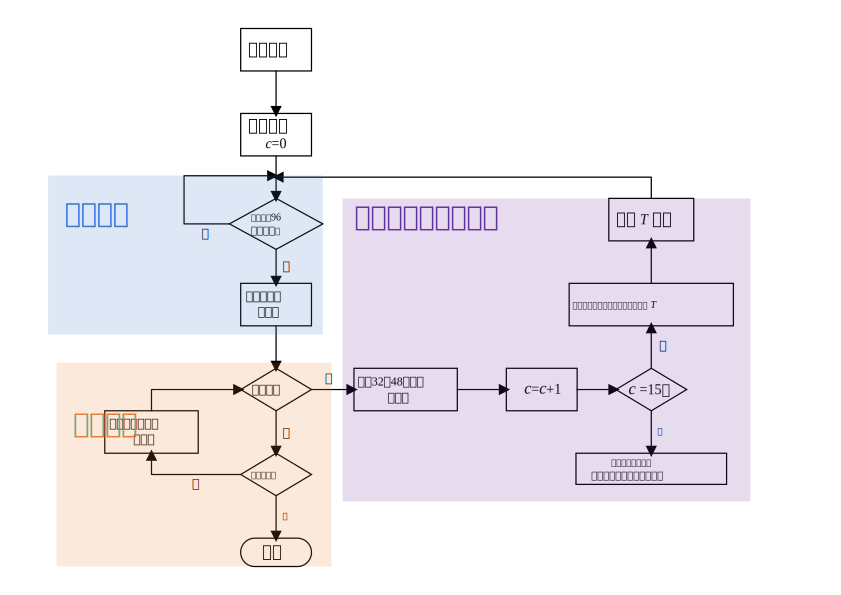
\includegraphics[width=0.75\textwidth]{img/3.4.2.1}
	\end{figure}

	帧接收流程:
	\begin{figure}[H]
		\centering
		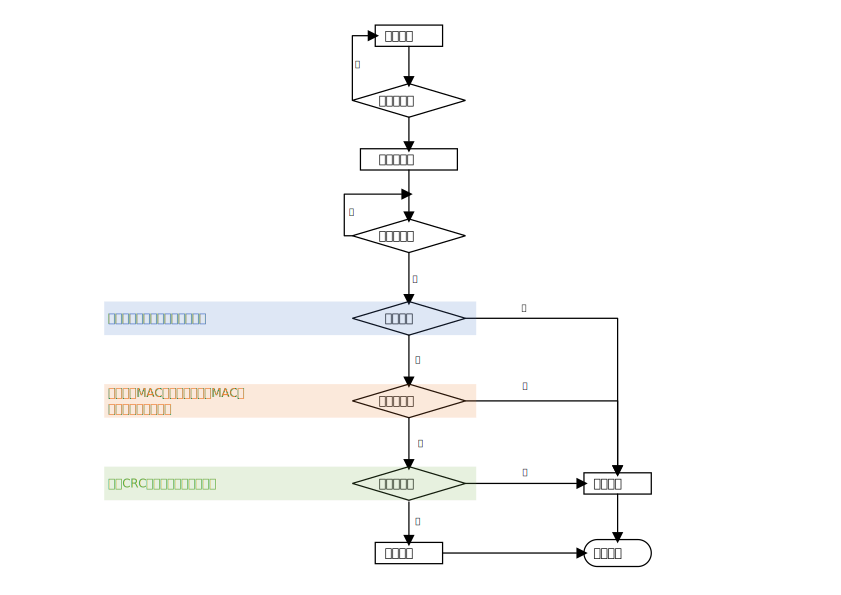
\includegraphics[width=0.7\textwidth]{img/3.4.2.2}
	\end{figure}

	\subsection{802.11 局域网的MAC层协议}

	\subsubsection{CSMA/CA协议}

	\begin{itemize}
		\item 在无线局域网中,仍然可以使用载波监听多址接入 CSMA , 即在发送帧之前先对传输媒体进行载波监听。若发现有其他站在发送帧,就推迟发送以免发生碰撞
		\item 在无线局域网中,不能使用碰撞检测CD ,原因如下:
		\begin{itemize}
			\item 由于无线信道的传输条件特殊,其信号强度的动态范围非常大,无线网卡上接收到的信号强度往往会远远小于发送信号的强度(可能相差百万倍)。如果要在无线网卡上实现碰撞检测CD ,对硬件的要求非常高
			\item 即使能够在硬件上实现无线局域网的碰撞检测功能,但由于无线电波传播的特殊性(存在隐蔽站问题), 进行碰撞检测的意义也不大
		\end{itemize}
	\end{itemize}

	\begin{figure}[H]
		\centering
		\includegraphics[width=0.85\textwidth]{img/3.4.3.1}
	\end{figure}

	\begin{itemize}
		\item 802.11 无线局域网使用 CSMA/CA 协议,在 CSMA 的基础上增加了一个碰撞避免 CA 功能,而不再实现碰撞检测功能
		\item 由于不可能避免所有的碰撞,并且无线信道误码率较高, 802.11 标准还使用了数据链路层确认机制(停止-等待协议) 来保证数据被正确接收
		\item 802.11 的 MAC 层标准定义了两种不同的媒体接入控制方式:
		\begin{itemize}
			\item 分布式协调功能 DCF(Distributed Coordination Function)。在 DCF 方式下,没有中心控制站点,每个站点使用 CSMA/CA 协议通过争用信道来获取发送权,这是802.11 定义的默认方式
			\item 点协调功能 PCF(Point Coordination Function)。PCF 方式使用集中控制的接入算法(一般在接入点AP 实现集中控制),是802.11 定义的可选方式,在实际中较少使用
		\end{itemize}
		\begin{figure}[H]
			\centering
			\includegraphics[width=0.5\textwidth]{img/3.4.3.2}
		\end{figure}
		\item 802.11 标准规定,所有的站点必须在持续检测到信道空闲一段指定时间后才能发送帧,这段时间称为帧间间隔IFS(InterFrame Space)
		\item 帧间间隔的长短取决于该站点要发送的帧的类型:
		\begin{itemize}
			\item 高优先级帧需要等待的时间较短,因此可优先获得发送权
			\item 优先级帧需要等待的时间较长。若某个站的低优先级帧还没来得及发送,而其他站的高优先级帧已发送到信道上,则信道变为忙态,因而低优先级帧就只能再推迟发送了。这样就减少了发生碰撞的机会
		\end{itemize}
		\item 常用的两种帧间间隔如下:
		\begin{itemize}
			\item 短帧间间隔 SIFS($28\mathrm{\mu s}$),是最短的帧间间隔,用来分隔开属于一次对话的各帧。一个站点应当能够在这段时间内从发送方式切换到接收方式。使用 SIFS 的帧类型有 ACK 帧、CTS 帧、由过长的 MAC 帧分片后的数据帧、以及所有回答 AP 探询的帧和在 PCF 方式中接入点 AP 发送出的任何帧
			\item DCF 帧间间隔 DIFS($128\mathrm{\mu s}$),它比短帧间间隔 SIFS 要长得多,在 DCF 方式中用来发送数据帧和管理帧
		\end{itemize}
	\end{itemize}

	CSMA/CA 协议工作原理:
	\begin{figure}[H]
		\centering
		\includegraphics[width=0.85\textwidth]{img/3.4.3.3}
	\end{figure}

	\begin{itemize}
		\item 当站点检测到信道是空闲的,并且所发送的数据帧不是成功发送完上一个数据帧之后立即连续发送的数据帧,
		则不使用退避算法
		\item 以下情况必须使用退避算法:
		\begin{itemize}
			\item 在发送数据帧之前检测到信道处于忙状态时
			\item 每一次重传一个数据帧时
			\item 在每一次成功发送后要连续发送下一个帧时(这是为了避免一个站点长时间占用信道)
		\end{itemize}
		\item 在执行退避算法时,站点为退避计时器设置一个随机的退避时间:
		\begin{itemize}
			\item 当退避计时器的时间减小到零时,就开始发送数据
			\item 当退避计时器的时间还未减小到零时而信道又转变为忙状态,这时就冻结退避计时器的数值,重新等待信道变为空闲,再经过时间 DIFS 后,继续启动退避计时器
		\end{itemize}
		\item 在进行第$i$次退避时,退避时间在时隙编号$\{1,2,\cdots, 2^{2+i}-1\}$中随机选择一个,然后乘以基本退避时间(也就是一个时隙的长度)就可以得到随机的退避时间。这样做是为了使不同站点选择相同退避时间的概率减少.当时隙编号达到255时(对应于第6次退避)就不再增加了
	\end{itemize}

	\begin{figure}[H]
		\centering
		\includegraphics[width=0.85\textwidth]{img/3.4.3.4}
	\end{figure}

	\subsubsection{对信道进行预约}

	\begin{itemize}
		\item 为了尽可能减少碰撞的概率和降低碰撞的影响, 802.11 标准允许要发送数据的站点对信道进行预约
		\begin{enumerate}[label=\arabic*.]
			\item 源站在发送数据帧之前先发送一个短的控制帧,称为请求发送 RTS(request to send),它包括源地址目的地址以及这次通信(包括相应的确认帧)所需的持续时间
			\item 若目的站正确收到源站发来的RTS帧,且媒体空闲,就发送一个响应控制帧,称为允许发送 CTS(clear to send),它也包括这次通信所需的持续时间(从 RTS 帧中将此持续时间复制到 CTS 帧中)
			\item 源站收到 CTS 帧后,再等待一段时间 SIFS 后,就可发送其数据帧
			\item 若目的站正确收到了源站发来的数据帧,在等待时间 SIFS 后,就向源站发送确认帧 ACK
		\end{enumerate}
		\begin{figure}[H]
			\centering
			\includegraphics[width=0.8\textwidth]{img/3.4.3.5}
		\end{figure}
		\item 除源站和目的站以外的其他各站,在收到 CTS 帧(或数据帧)后就推迟接入到无线局域网中。这样就保证了源站和目的站之间的通信不会受到其他站的干扰
		\item 如果 RTS 帧发生碰撞,源站就收不到 CTS 帧,需执行退避算法重传 RTS 帧
		\item 由于RTS帧和CTS帧很短,发送碰撞的概率、碰撞产生的开销及本身的开销都很小。而对于一般的数据帧,其发送时延往往大于传播时延(因为是局域网),碰撞的概率很大,且一旦发生碰撞而导致数据帧重发,则浪费的时间就很多,因此用很小的代价对信道进行预约往往是值得的。802.11 标准规定了3种情况供用户选择:
		\begin{itemize}
			\item 使用 RTS 帧和 CTS 帧
			\item 不使用 RTS 帧和 CTS 帧
			\item 只有当数据帧的长度超过某一数值时才使用 RTS 帧和 CTS 帧
		\end{itemize}
		\item 除 RTS 帧和 CTS 帧会携带通信需要持续的时间,数据帧也能携带通信需要持续的时间,这称为802.11的虚拟载波监听机制
		\item 由于利用虚拟载波监听机制, 站点只要监听到 RTS 帧、CTS 帧或数据帧中的任何一个,就能知道信道被占用的持续时间,而不需要真正监听到信道上的信号,因此虚拟载波监听机制能减少隐蔽站带来的碰撞问题
	\end{itemize}

	CSMA/CA的基本流程图:
	\begin{figure}[H]
		\centering
		\includegraphics[width=0.68\textwidth]{img/3.4.3.6}
	\end{figure}

	\subsection{使用集线器的星形拓扑}

	\begin{figure}[H]
		\centering
		\includegraphics[width=0.5\textwidth]{img/3.19}
	\end{figure}

	集线器(hub)的一些特点如下:
	\begin{itemize}
		\item 使用集线器的以太网在逻辑上仍是一个总线网,各站共享逻辑上的总线,使用的还是 CSMA/CD 协议(更具体些说,是各站中的适配器执行 CSMA/CD 协议)。网络中的各站必须竞争对传输媒体的控制,并且在同一时刻至多只允许一个站发送数据
		\item 一个集线器有许多接口,每个接口通过 RJ-45 插头用两对双绞线与一台计算机上的适配器相连,一个集线器很像一个多接口的转发器
		\item 集线器工作在物理层,它的每个接口仅仅简单地转发比特,不进行碰撞检测
		\item 集线器一般都有少量的容错能力和网络管理功能。例如,若网络中某个网卡出了故障,不停地在发送帧,此时集线器可以检测到这个问题,在内部断开与出故障网卡的连线,使整个以太网仍能正常工作
	\end{itemize}

	\subsection{以太网的信道利用率}
	\begin{figure}[H]
		\centering
		\includegraphics[width=0.6\textwidth]{img/3.21}
	\end{figure}
	考虑上图的以太网信道被占用的情况
	\begin{itemize}
		\item 一个站在发送帧时出现碰撞,经过一个争用期 $2 \tau$ 后,可能又出现了碰撞,这样经过若干个争用期后,一个站发送成功了
		\item 假定发送帧需要的时间是 $T_0$ ,等于帧长除以发送速率
		\item 考虑在最极端情况下,发送站在传输媒体的一端,当发送站发送完最后一个比特是,这个比特在在以太网上传播需要的时间为 $\tau$ 
		\item 所以必须在经过时间 $T_0 + \tau $ 后以太网的媒体才完全进入空闲状态,允许其他站发送数据
	\end{itemize}

	定义参数 $a$ 为以太网单程端到端时延 $\tau$ 与帧的发送时间 $T_0$ 之比$$a = \frac{\tau}{T_0}$$
	\begin{itemize}
		\item 参数 $a$ 越大,表明争用期所占的比例越大,这就使得每发生一次碰撞就浪费了不少的信道资源,使得信道利用率明显降低
		\item 当数据率一定时,以太网的连线的长度受到限制,同时以太网的帧长不能太短
	\end{itemize}

	以太网极限信道利用率 $S_{max}$ 为
	$$S_{\mathrm{max}} = \frac{T_0}{T_0 + \tau} = \frac{1}{1+a}$$
	\begin{itemize}
		\item 只有当参数 $a$ 远小于 1 才能得到尽可能高的极限信道利用率
	\end{itemize}

	\subsection{以太网的MAC层}

	\subsubsection{MAC层的硬件地址}

	\begin{itemize}
		\item 当多个主机连接在同一个广播信道上,要想实现两个主机之间的通信,则每个主机都必须有一个唯一的标识,即一个数据链路层地址
		\item 在每个主机发送的帧中必须携带标识发送主机和接收主机的地址。由于这类地址是用于媒体介入控制 MAC(media access control),因此这类地址被称为 MAC 地址
		\begin{itemize}
			\item MAC 地址一般被固化在网卡(网络适配器)的电可擦可编程只读存储器 EEPROM 中,因此 MAC 地址也被称为硬件地址
			\item MAC 地址有时也被称为物理地址,但这并不意味着 MAC 地址属于网络体系结构中的物理层
		\end{itemize}
		\item 一般情况下,用户主机会包含两个网络适配器:有线局域网适配器(有线网卡)和无线局域网适配器(无线网卡)。每个网络适配器都有一个全球唯一的 MAC 地址。而交换机和路由器往往拥有更多的网络接口,所以会有更多的 MAC 地址。所以,严格来说,MAC 地址是对网络上各接口的唯一标识,而不是对网络上各设备的唯一标识
		\item IEEE 802 局域网的 MAC 帧格式
		\begin{figure}[H]
			\centering
			\includegraphics[width=0.7\textwidth]{img/3.4.5.1}
		\end{figure}
		\begin{itemize}
			\item IEEE 的注册管理机构 RA(Registration Authority)是局域网全球地址的法定管理机构,负责分配地址字段的 6 个字节中的前三个字节(即高位 24 位)。世界上凡要生产局域网适配器的厂家都必须向 IEEE 购买由这三个字节构成的地址块,称为组织唯一标识符 OUI(organizationally unique identifier)
			\item 地址字段中的后三个字节(即低位 24 位)则由厂家自行指派,称为扩展标识符(extended identifier),只要保证生产出的适配器没有重复地址即可
			\item 地址字段的第一字节的最低位为 I/G(Individual/Group)位,当 I/G 位为 0 时,地址字段表示一个单个站地址;当 I/G 位为 1 时表示组地址,用来进行多播
			\item 地址字段第 1 字节的最低第二位规定为 G/L(Global/Local) 位。当 G/L 位为 0 时是全球管理(保证 在全球没有相同的地址),厂商向 IEEE 购买的 OUI 都属于全球管理。当地址字段的 G/L 位为 1 时是本地管理,这时用户可任意分配网络上的地址
		\end{itemize}
	\end{itemize}


	\subsubsection{MAC帧的格式}

	\begin{figure}[H]
		\centering
		\includegraphics[width=0.8\textwidth]{img/3.22}
	\end{figure}

	\begin{itemize}
		\item 以太网 V2的 MAC 帧格式为
		\begin{itemize}
			\item 前两个字段分别为6字节长的目的地址和源地址字段
			\item 第三个字端是 2 字节的类型字段,用来标志上一层使用的是什么协议,以便把收到的 MAC 帧的数据上交给上一层的这个协议
			\item 第四个字段是数据字段,其长度在 46 到 1500 字节之间(最小长度 64 字节减去 18 字节的首部和尾部就得出数据字段的最小长度 46 字节)
			\item 最后一个字段是 4 字节的帧检验序列 FCS(使用 CRC 检验)
		\end{itemize}
		\item 在以太网 V2 的 MAC 帧格式中,其首部并没有一个帧长度(或数据长度)字段。那么,MAC 子层又怎样知道从接收到的以太网帧中取出多少字节的数据交付上一层协议呢?
		\begin{itemize}
			\item 曼彻斯特编码的 一个重要特点就是:在曼彻斯特编码的每一个码元(不管码元是 1 或 0)的正中间一定有一 次电压的转换(从高到低或从低到高)。当发送方把一个以太网帧发送完毕后,就不再发送其他码元了(既不发送 1,也不发送 0)。因此,发送方网络适配器的接口上的电压也就不再变化了。这样,接收方就可以很容易地找到以太网帧的结束位置。在这个位置往前数 4 字节(FCS 字段长度是 4 字节),就能确定数据字段的结束位置
		\end{itemize}
		\item 当数据字段的长度小于 46 字节时,MAC 子层就会在数据字段的后面加入一个整数字节的填充字段,以保证以太网的 MAC 帧长不小于 64 字节
		\begin{itemize}
			\item 上层协议如何知道填充字段的长度呢:当上层使用 IP 协议时,其首部就有一个“总长度”字段。因此,“总长度”加上填充字段的长度,应当等于 MAC 帧数据字段的长度。例如,当 IP 数据报的总长度为 42 字节时,填充字段共有 4 字节。当 MAC 帧把 46 字节的数据上交给 IP 层后,IP 层就把其中最后 4 字节的填充字段丢弃
		\end{itemize}
	\end{itemize}

	\section{拓展的以太网}

	\subsection{在物理层拓展以太网}

	如果使用多个集线器,就可以连接成覆盖更大范围的多级星形结构的以太网

	\begin{figure}[H]
		\centering
		\includegraphics[width=0.7\textwidth]{img/3.24}
	\end{figure}

	\subsection{在数据链路层拓展以太网}
	
	\subsubsection{以太网交换机的特点}

	\begin{itemize}
		\item 以太网交换机实质上就是一个多接口的网桥,每个接口都可以直接与一台主机或另一个以太网交换机相连,一般都工作在全双工方式
		\item 以太网交换机具有并行性,能同时连通多对接口,使多对主机能同时通信,相互通信的主机都是独占传输媒体,无碰撞地传输数据(不使用 CSMA/CD 协议)
		\item 以太网交换机一般都具有多种速率的接口,例如10Mb/s、100Mb/s、1Gb/s和10Gb/s接口的多种组合
		\item 以太网交换机工作在数据链路层(也包括物理层),它收到帧后,在帧交换表中查找帧的目的 MAC 地址所对应的接口号,然后通过该接口转发帧
		\item 以太网交换机是一种即插即用设备,其内部的帧交换表是通过自学习算法自动地逐渐建立起来的
		\item 帧的转发方式
		\begin{itemize}
			\item 大多以太网交换机采用存储转发方式
			\item 一些交换机采用直通交换的方式:采用基于硬件的交叉矩阵,交换时延非常小,但不检查帧是否有差错
		\end{itemize}
	\end{itemize}

	\begin{figure}[H]
		\centering
		\includegraphics[width=0.75\textwidth]{img/3.25}
	\end{figure}

	\subsection{以太网交换机的自学习功能}
	以上图为例说明以太网交换机是怎样进行自学习的
	\begin{itemize}
		\item A 先向 B 发送一帧,从接口1进入到交换机。交换机收到帧后,先查找交换表,没有查到应从哪个接口转发这个帧
		\item 接着,交换机把这个帧的源地址 A 和接口1写入交换表中,并向除接口1以外的所有接口广播这个帧
		\item C 和 D 将丢弃这个帧,因为目的地址不对。只 B 才收下这个目的地址正确的帧。这也称为过滤
		\item 假定接下来 B 通过接口3向 A 发送一帧。交换机查找交换表,发现交换表中的 MAC 地址有 A。表明要发送给 A 的帧应从接口 1 转发
		\item 于是就把这个帧传送到接口 1 转发给 A
		\item 考虑到有时可能要在交换机的接口更换主机,或者主机要更换其网络适配器,这就需要更改交换表中的项目。为此,在交换表中每个项目都设有一定的有效时间,过期的项目就自动被删除。用这样的方法保证交换表中的数据都符合当前网络的实际状况
	\end{itemize}

	\textbf{例:}为简单起见,主机 A、B、C、D、E、F、G、H 的 MAC 地址与其主机名称相同,主机间依次入如下通信:B $\rightarrow$ C、D $\rightarrow$ A、G $\rightarrow$ D、E $\rightarrow$ H、C $\rightarrow$ B 和 F $\rightarrow$ G。请给出以太网交换机1,2,3的自学习过程以及各自最终的帧交换表的内容

	\begin{figure}[H]
		\centering
		\includegraphics[width=0.8\textwidth]{img/3.5.2.2.1}
	\end{figure}

	自学习过程如下:
	\begin{table}[H]
		\centering
		\begin{tabular}{|c|c|c|c|}
		\hline
		通信过程              & 以太网交换机1 & 以太网交换机2 & 以太网交换机3 \\ \hline
		B $\rightarrow$ C & 登记,盲目转发 & 登记,盲目转发 & 登记,盲目转发 \\ \hline
		D $\rightarrow$ A             & 登记,盲目转发 & 登记,盲目转发 & 登记,盲目转发 \\ \hline
		G $\rightarrow$ D             & 收不到     & 登记,明确转发 & 登记,明确转发 \\ \hline
		E $\rightarrow$ H             & 登记,盲目转发 & 登记,盲目转发 & 登记,盲目转发 \\ \hline
		C $\rightarrow$ B             & 登记,明确转发 & 收不到     & 收不到     \\ \hline
		F $\rightarrow$ G             & 收不到     & 收不到     & 登记,明确转发 \\ \hline
		\end{tabular}
	\end{table}

	最终的帧交换表如下:
	\begin{figure}[H]
		\centering
		\includegraphics[width=0.8\textwidth]{img/3.5.2.2.2}
	\end{figure}

	\begin{itemize}
		\item 有时为了增加网络的可靠性,在使用以太网交换机组网时,往往会增加一些冗余的链路
		\item 但是冗余链路会形成网络环路,造成广播风暴,主机收到重复的广播帧以及交换机的帧交换表震荡(漂移)等问题
	\end{itemize}

	\begin{figure}[H]
		\centering
		\includegraphics[width=0.5\textwidth]{img/3.26}
	\end{figure}

	\begin{itemize}
		\item 以太网交换机使用生成树协议 STP(spanning tree protocol),可以在增加冗余链路来提高网络可靠性的同时又避免网络环路带来的各种问题
		\begin{itemize}
			\item 不论交换机之间采用怎样的物理连接,交换机都能自动计算并构建一个逻辑上没有环路的网络,其拓扑结构必须是树形的
			\item 最终生成的树形拓扑结构要确保连通整个网络
			\item 当首次连接交换机或网络物理拓扑发生变化时(有可能是人为改变或故障),交换机都将进行生成树的重新计算
		\end{itemize}
	\end{itemize}

	\subsection{虚拟局域网}
	
	\begin{itemize}
		\item 虚拟局域网 VLAN 是由一些局域网网段构成的与物理位置无关的逻辑组,而这些网段具有某些共同的需求。每一个 VLAN 的帧都有一个明确的标识符,指明发送这个帧的计算机属于哪一个 VLAN
		\item 虚拟局域网只是局域网给用户提供的一种服务,而并不是一种新型局域网
		\begin{figure}[H]
			\centering
			\includegraphics[width=0.6\textwidth]{img/3.27}
		\end{figure}
		\item 在虚拟局域网上的每一个站都可以收到同一个虚拟局域网上的其他成员所发出的广播
		\begin{itemize}
			\item 当 $B_1$ 向工作组内成员发送数据时,计算机 $B_2$ 和 $B_3$ 将会收到广播的信息,虽然它们没有和 $B_1$ 连在同一个以太网交换机上
			\item 当 $B_1$ 向工作组内成员发送数据时,计算机 $A_1$,$A_2$ 和 $C_1 $ 都不会收到 $B_1$ 发出的广播信息,虽然它们都与 $B_1$ 连接在同一个以太网交换机上
		\end{itemize}
		\item 虚拟局域网限制了接收广播信息的计算机数,使得网络不会因传播过多的广播信息(即所谓的“广播风暴”)而引起性能恶化
		\begin{figure}[H]
			\centering
			\includegraphics[width=0.75\textwidth]{img/3.28}
		\end{figure}
		\item 虚拟局域网协议允许在以太网的帧格式中插入一个 4 字节的标识符,称为 VLAN 标记,用来指明发送该帧的计算机属于哪一个虚拟局域网
		\item 插入 VLAN 标记得出的帧称为 802.1Q 帧
		\item VLAN 标记字段的长度是 4 字节,插入在以太网 MAC 帧的源地址字段和类型字段之间
		\item VLAN 标记的前两个字节总是设置为\ \verb|0x8100|,称为 IEEE 802.1Q 标记类型
		\item 当数据链路层检测到 MAC 帧的源地址字段后面的两个字节的值是 \ \verb|0x8100|\ 时,就知道现在插入了 4 字节的 VLAN 标记。于是就接着检查后面两个字节的内容。在后面的两个字节中,前 3 位是用户优先级字段,接着的一位是规范格式指示符 CFI(Canonical Format Indicator),最后的12位是该虚拟局域网VLAN标识符VID,它唯一地标志了这个以太网帧属于哪一个 VLAN
		\item 由于用于 VLAN 的以太网帧的首部增加了 4 个字节,因此以太网的最大帧长从原来的 1518 字节(1500 字节的数据加上 18 字节的首部)变为 1522 字节
	\end{itemize}





\end{document}


